\documentclass[12pt, a4paper]{article}
\usepackage[utf8]{inputenc}
\usepackage[french]{babel}
\usepackage{graphicx}
\usepackage{geometry}
\usepackage{hyperref}
\usepackage{listings}
\usepackage{xcolor}
\usepackage{booktabs}
\usepackage{float}

% Configuration de la page
\geometry{top=2.5cm, bottom=2.5cm, left=2.5cm, right=2.5cm}

% Configuration des liens
\hypersetup{
    colorlinks=true,
    linkcolor=black,
    filecolor=magenta,      
    urlcolor=blue,
    pdftitle={Rapport TP Deep Learning - Segmentation},
}

% Configuration du style pour le code Python
\definecolor{codegreen}{rgb}{0,0.6,0}
\definecolor{codegray}{rgb}{0.5,0.5,0.5}
\definecolor{codepurple}{rgb}{0.58,0,0.82}
\definecolor{backcolour}{rgb}{0.95,0.95,0.92}

\lstset{
    language=Python,
    backgroundcolor=\color{backcolour},   
    commentstyle=\color{codegreen},
    keywordstyle=\color{blue},
    numberstyle=\tiny\color{codegray},
    stringstyle=\color{codepurple},
    basicstyle=\ttfamily\footnotesize,
    breakatwhitespace=false,         
    breaklines=true,                 
    captionpos=b,                    
    keepspaces=true,                 
    numbers=left,                    
    numbersep=5pt,                  
    showspaces=false,                
    showstringspaces=false,
    showtabs=false,                  
    tabsize=2,
    frame=single
}

\begin{document}

% ==========================================
% PAGE DE GARDE
% ==========================================
\begin{titlepage}
    \centering
    \vspace*{0.5cm}
    
    {\Large \textbf{Université Sultan Moulay Slimane}}\\
    \vspace{0.2cm}
    {\large \textbf{Faculté des Sciences et Techniques - Béni Mellal}}\\
    \vspace{2cm}
    
    {\Large \textbf{Master AIDC 2025–2026}}\\
    \vspace{2cm}
    
    \rule{\textwidth}{1pt}
    \vspace{0.6cm}
    {\huge \textbf{Rapport de Travaux Pratiques}}\\
    \vspace{0.4cm}
    {\Large \textbf{Deep Learning : Segmentation Sémantique}}\\
    \vspace{0.3cm}
    {\large Architecture U-Net \& Transfer Learning (ResNet-34)}\\
    \vspace{0.4cm}
    \rule{\textwidth}{1pt}
    
    \vspace{3cm}
    
    \begin{minipage}{0.4\textwidth}
        \begin{flushleft} \large
            \emph{Réalisé par :}\\
            \textbf{Votre Nom et Prénom} % <--- METTEZ VOTRE NOM ICI
        \end{flushleft}
    \end{minipage}
    \hfill
    \begin{minipage}{0.4\textwidth}
        \begin{flushright} \large
            \emph{Encadré par :} \\
            \textbf{Nom du Professeur} % <--- METTEZ LE NOM DU PROF ICI
        \end{flushright}
    \end{minipage}
    
    \vfill
    
    {\normalsize Année universitaire : 2025 / 2026}
\end{titlepage}

% ==========================================
% TABLE DES MATIÈRES
% ==========================================
\tableofcontents
\newpage

% ==========================================
% INTRODUCTION
% ==========================================
\section{Introduction}
Ce rapport présente la mise en œuvre et l'analyse détaillée des expérimentations menées sur la tâche de segmentation sémantique d'images dans le cadre des travaux pratiques de Deep Learning. L'objectif principal est de classifier chaque pixel d'une image selon trois classes définies : l'animal (classe d'intérêt), le contour de l'animal, et le fond (arrière-plan). 

Pour ce faire, nous exploitons le dataset d'images d'animaux domestiques \textit{Oxford-IIIT Pet}. Nous commençons par analyser les caractéristiques du dataset avant de concevoir et d'évaluer une architecture \textit{U-Net} construite "from scratch". Dans un second temps, nous optimisons cette segmentation à travers une approche de \textit{Transfer Learning} en utilisant le modèle \textit{ResNet-34} pré-entraîné sur ImageNet comme encodeur. Les performances de ces différents modèles sont comparées à l'aide de métriques rigoureuses de performance et de vitesse.

\newpage
% ==========================================
% EXERCICE 1 - SEGMENTATION
% ==========================================
\section{Exercice 1 — Segmentation Sémantique}

\subsection{Partie 1 : Dataset Oxford-IIIT Pet}

\subsubsection*{Chargement, visualisation et distribution des classes}
Pour le traitement des images et la gestion des masques de segmentation, nous utilisons la classe personnalisée \texttt{PetSegmentationDataset} dérivée de PyTorch.

\begin{figure}[H]
    \centering
    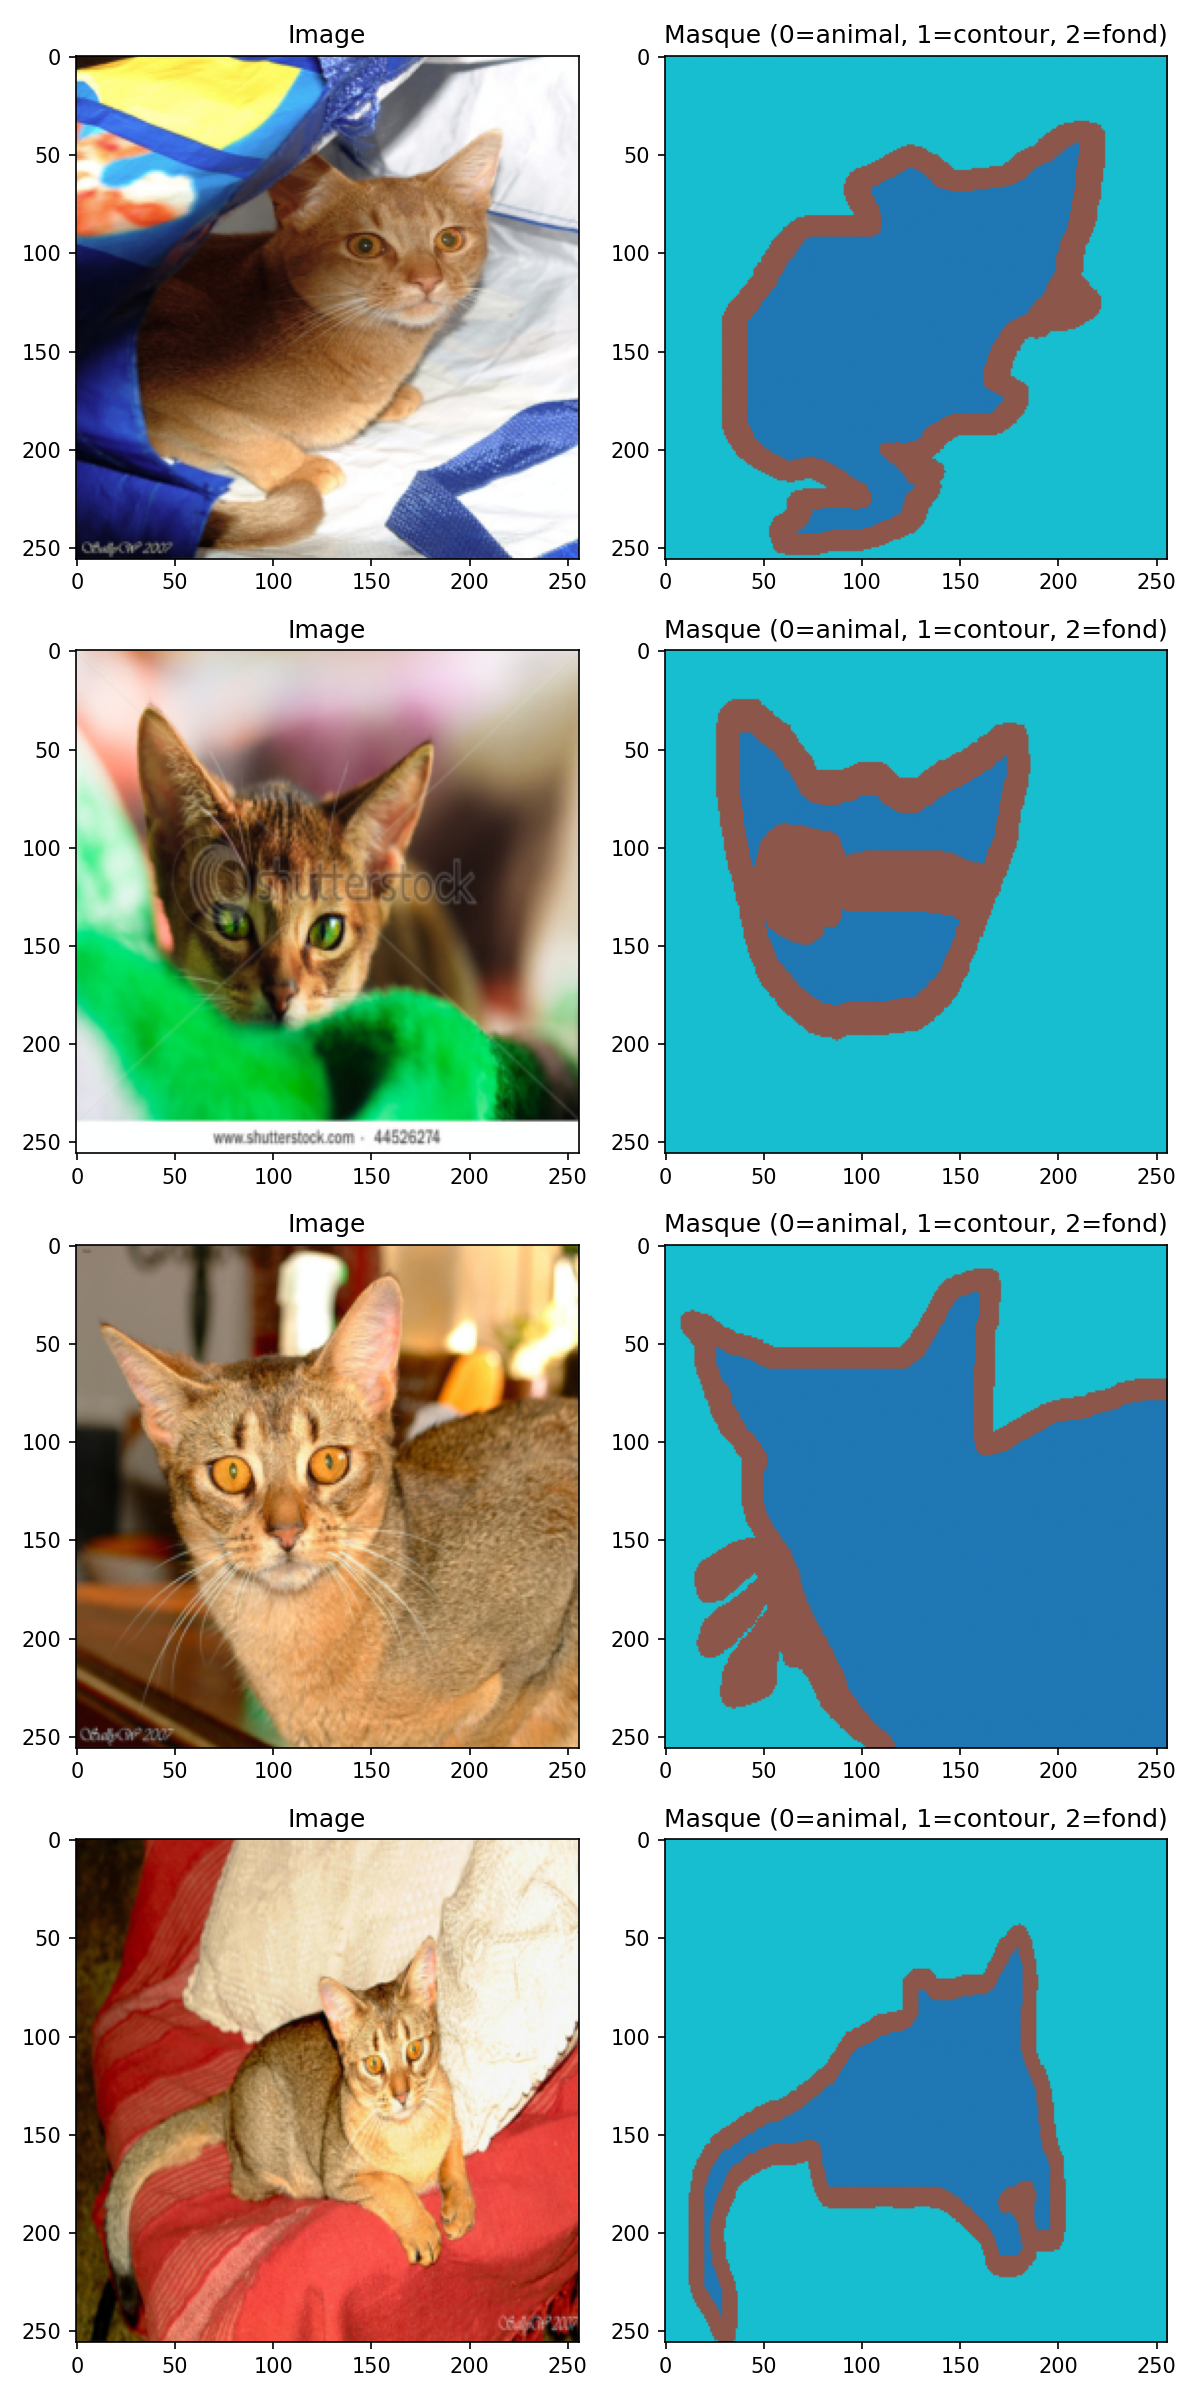
\includegraphics[width=0.75\textwidth]{visualisation_dataset.png}
    \caption{Visualisation de quelques exemples d'images et leurs masques de segmentation correspondants.}
\end{figure}

L'évaluation de la distribution spatiale des pixels sur un échantillon représentatif de 500 images du jeu de données révèle les proportions suivantes :
\begin{itemize}
    \item \textbf{Animal (classe 0) :} 28.3 \% des pixels
    \item \textbf{Contour (classe 1) :} 12.0 \% des pixels
    \item \textbf{Fond (classe 2) :} 59.6 \% des pixels
\end{itemize}

\textbf{Analyse du déséquilibre :} 
Ces statistiques démontrent que la classe \textit{contour} est très minoritaire par rapport aux autres classes, tandis que le \textit{fond} représente la majorité absolue de l'espace d'image. Ce déséquilibre constitue un écueil classique en segmentation : un modèle naïf cherchant uniquement à réduire le taux d'erreur global aura tendance à ignorer les contours pour se focaliser sur les zones d'arrière-plan faciles à classer. Il est donc indispensable d'introduire des techniques adaptées telles que la pondération par classe dans la fonction de perte Cross-Entropy ou l'utilisation de la Dice Loss.

\subsubsection*{Augmentation de données synchronisée}
Afin de régulariser notre modèle et d'améliorer sa généralisation, nous appliquons une fonction d'augmentation géométrique et photométrique. Étant en segmentation, il est capital que les transformations géométriques s'appliquent identiquement à l'image et au masque (target).

\begin{lstlisting}[caption={Implémentation de l'augmentation synchronisée}]
class SyncAugmentation:
    def __init__(self, p=0.5):
        self.p = p

    def __call__(self, img, mask):
        if random.random() < self.p:
            img, mask = TF.hflip(img), TF.hflip(mask)
        if random.random() < self.p:
            angle = random.uniform(-15, 15)
            img = TF.rotate(img, angle)
            # NEAREST est crucial pour ne pas creer de fausses classes !
            mask = TF.rotate(mask, angle, interpolation=TF.InterpolationMode.NEAREST)
        if random.random() < self.p:
            img = transforms.ColorJitter(brightness=0.3, contrast=0.3, saturation=0.2)(img)
        return img, mask
\end{lstlisting}

\textbf{Justification de l'interpolation NEAREST :} 
Lors de l'application d'une rotation sur le masque, l'interpolation par défaut (comme le bilinéaire) effectuerait des moyennes pondérées des indices de classes aux frontières (par exemple, interpoler entre la classe 0 et la classe 2 produirait une classe 1 factice). L'utilisation de \texttt{TF.InterpolationMode.NEAREST} garantit que chaque pixel du masque transformé conserve rigoureusement une valeur entière discrète correspondant à l'une des trois classes initiales. Par ailleurs, la transformation de couleur \texttt{ColorJitter} ne s'applique que sur l'image car modifier la couleur des pixels du masque n'a aucun sens sémantique.

\begin{figure}[H]
    \centering
    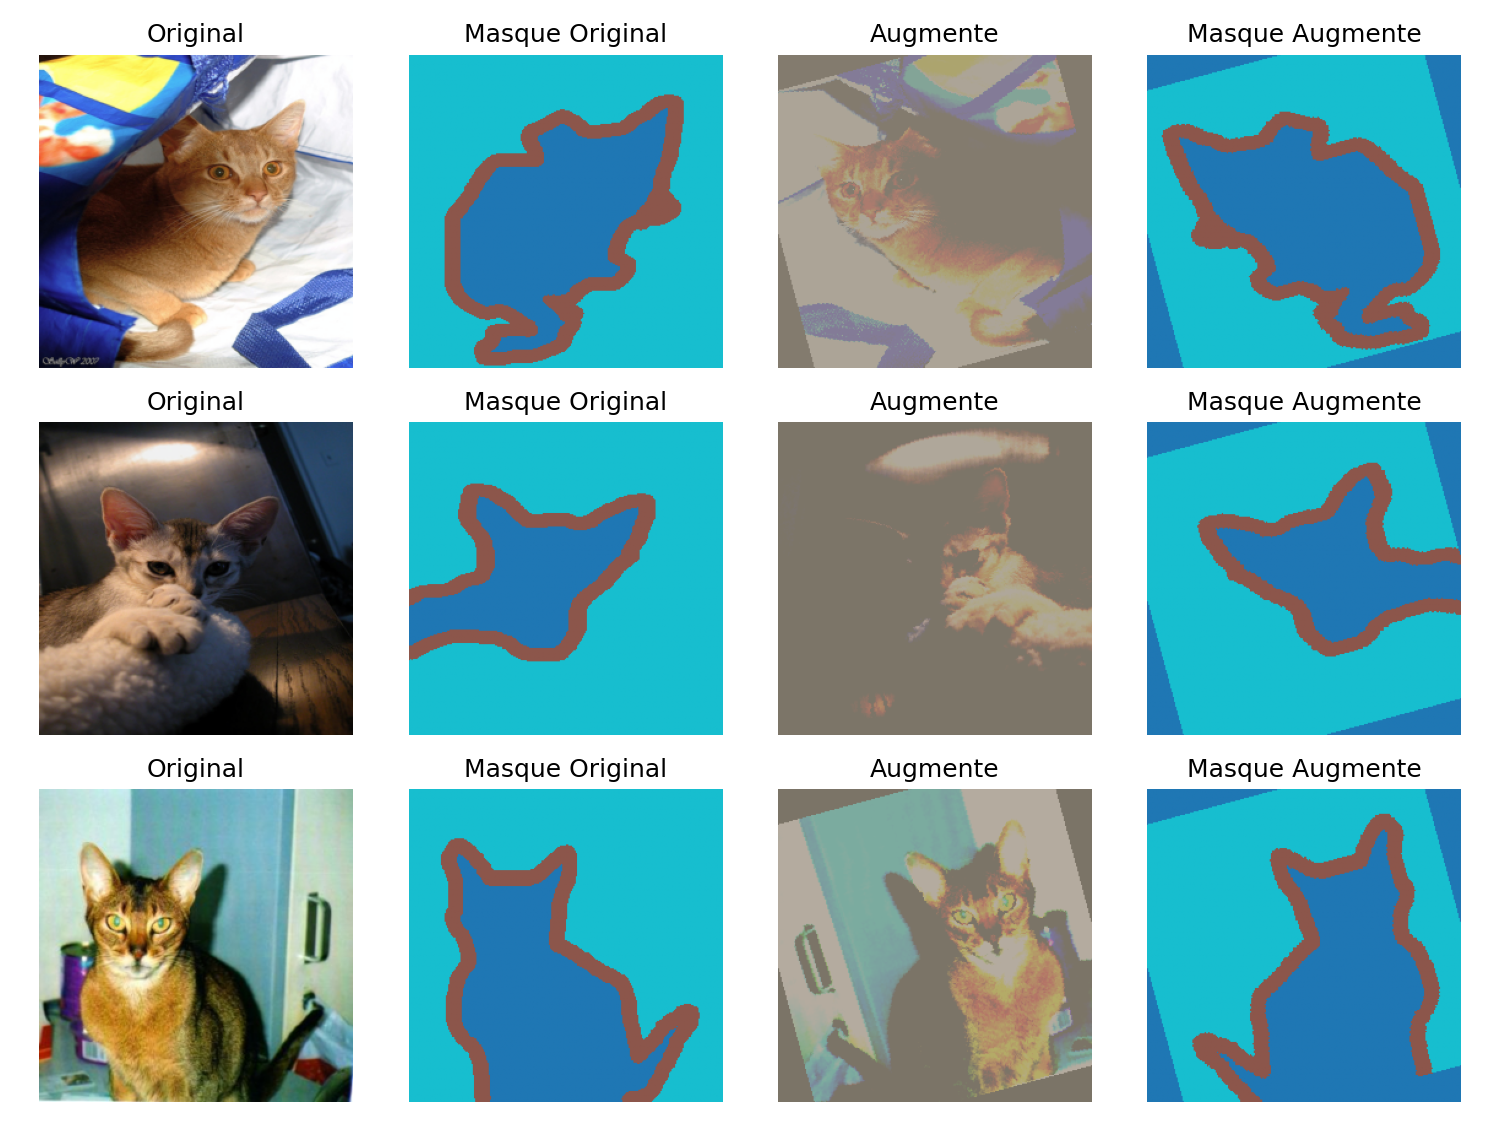
\includegraphics[width=0.85\textwidth]{augmentation_comparison.png}
    \caption{Visualisation comparée d'exemples originaux (image et masque GT) et leurs versions augmentées correspondantes après application des transformations géométriques et photométriques (rotation, flip horizontal et jitter de couleur).}
\end{figure}

\subsubsection*{DataLoaders et configuration du Batch Size}
Le dataset (3680 images au total) est divisé de manière aléatoire selon une répartition stricte 70\%/15\%/15\% :
\begin{itemize}
    \item \textbf{Train set :} 2576 images (avec augmentation de données)
    \item \textbf{Validation set :} 552 images
    \item \textbf{Test set :} 552 images
\end{itemize}

\textbf{Justification du Batch Size :} 
Nous avons fixé le batch size à $8$. Ce choix découle d'un compromis entre la stabilité des gradients et les contraintes de mémoire VRAM de la carte graphique locale. Chaque image de taille $256 \times 256 \times 3$ codée sur 32 bits représente environ $768$ Ko. Pour un batch de 8, la taille mémoire brute des données d'entrée est minime ($\approx 6.1$ Mo). Cependant, lors des étapes de propagation avant (forward pass), les cartes d'activation générées par chaque couche de convolution doivent être stockées pour le calcul des gradients (backpropagation), ce qui multiplie l'empreinte mémoire par un facteur important. Un batch size de 8 permet de garantir que l'entraînement s'exécute sans dépassement de mémoire (Out-Of-Memory) tout en profitant pleinement de la parallélisation CUDA.

\subsection{Partie 2 : SimpleUNet}

\subsubsection*{Architecture et paramètres du modèle}
Le modèle \texttt{SimpleUNet} a été entièrement codé de zéro. Avec une structure à 4 niveaux d'encodage/décodage et un nombre de filtres de départ à $base\_features=32$, il compte au total \textbf{1,949,763 paramètres entraînables}. C'est une architecture légère et rapide, idéale pour établir une référence (baseline) sur cette tâche.

La structure détaillée du réseau générée par l'outil \texttt{torchinfo} pour une entrée de dimensions $(1, 3, 256, 256)$ est présentée ci-dessous :

\begin{lstlisting}[basicstyle=\ttfamily\tiny, caption={Dimensions des tenseurs et paramètres couche par couche pour SimpleUNet}]
==========================================================================================
Layer (type:depth-idx)                   Output Shape              Param #
==========================================================================================
SimpleUNet                               [1, 3, 256, 256]          --
├─ConvBlock: 1-1                         [1, 32, 256, 256]         --
│    └─Sequential: 2-1                   [1, 32, 256, 256]         --
│    │    └─Conv2d: 3-1                  [1, 32, 256, 256]         896
│    │    └─BatchNorm2d: 3-2             [1, 32, 256, 256]         64
│    │    └─ReLU: 3-3                    [1, 32, 256, 256]         --
│    │    └─Conv2d: 3-4                  [1, 32, 256, 256]         9,248
│    │    └─BatchNorm2d: 3-5             [1, 32, 256, 256]         64
│    │    └─ReLU: 3-6                    [1, 32, 256, 256]         --
├─MaxPool2d: 1-2                         [1, 32, 128, 128]         --
├─ConvBlock: 1-3                         [1, 64, 128, 128]         --
│    └─Sequential: 2-2                   [1, 64, 128, 128]         --
│    │    └─Conv2d: 3-7                  [1, 64, 128, 128]         18,496
│    │    └─BatchNorm2d: 3-8             [1, 64, 128, 128]         128
│    │    └─ReLU: 3-9                    [1, 64, 128, 128]         --
│    │    └─Conv2d: 3-10                 [1, 64, 128, 128]         36,928
│    │    └─BatchNorm2d: 3-11            [1, 64, 128, 128]         128
│    │    └─ReLU: 3-12                   [1, 64, 128, 128]         --
├─MaxPool2d: 1-4                         [1, 64, 64, 64]           --
├─ConvBlock: 1-5                         [1, 128, 64, 64]          --
│    └─Sequential: 2-3                   [1, 128, 64, 64]          --
│    │    └─Conv2d: 3-13                 [1, 128, 64, 64]          73,856
│    │    └─BatchNorm2d: 3-14            [1, 128, 64, 64]          256
│    │    └─ReLU: 3-15                   [1, 128, 64, 64]          --
│    │    └─Conv2d: 3-16                 [1, 128, 64, 64]          147,584
│    │    └─BatchNorm2d: 3-17            [1, 128, 64, 64]          256
│    │    └─ReLU: 3-18                   [1, 128, 64, 64]          --
├─MaxPool2d: 1-6                         [1, 128, 32, 32]          --
├─ConvBlock: 1-7                         [1, 256, 32, 32]          --
│    └─Sequential: 2-4                   [1, 256, 32, 32]          --
│    │    └─Conv2d: 3-19                 [1, 256, 32, 32]          295,168
│    │    └─BatchNorm2d: 3-20            [1, 256, 32, 32]          512
│    │    └─ReLU: 3-21                   [1, 256, 32, 32]          --
│    │    └─Conv2d: 3-22                 [1, 256, 32, 32]          590,080
│    │    └─BatchNorm2d: 3-23            [1, 256, 32, 32]          512
│    │    └─ReLU: 3-24                   [1, 256, 32, 32]          --
├─Upsample: 1-8                          [1, 256, 64, 64]          --
├─ConvBlock: 1-9                         [1, 128, 64, 64]          --
│    └─Sequential: 2-5                   [1, 128, 64, 64]          --
│    │    └─Conv2d: 3-25                 [1, 128, 64, 64]          442,496
│    │    └─BatchNorm2d: 3-26            [1, 128, 64, 64]          256
│    │    └─ReLU: 3-27                   [1, 128, 64, 64]          --
│    │    └─Conv2d: 3-28                 [1, 128, 64, 64]          147,584
│    │    └─BatchNorm2d: 3-29            [1, 128, 64, 64]          256
│    │    └─ReLU: 3-30                   [1, 128, 64, 64]          --
├─Upsample: 1-10                         [1, 128, 128, 128]        --
├─ConvBlock: 1-11                        [1, 64, 128, 128]         --
│    └─Sequential: 2-6                   [1, 64, 128, 128]         --
│    │    └─Conv2d: 3-31                 [1, 64, 128, 128]         110,656
│    │    └─BatchNorm2d: 3-32            [1, 64, 128, 128]         128
│    │    └─ReLU: 3-33                   [1, 64, 128, 128]         --
│    │    └─Conv2d: 3-34                 [1, 64, 128, 128]         36,928
│    │    └─BatchNorm2d: 3-35            [1, 64, 128, 128]         128
│    │    └─ReLU: 3-36                   [1, 64, 128, 128]         --
├─Upsample: 1-12                         [1, 64, 256, 256]         --
├─ConvBlock: 1-13                        [1, 32, 256, 256]         --
│    └─Sequential: 2-7                   [1, 32, 256, 256]         --
│    │    └─Conv2d: 3-37                 [1, 32, 256, 256]         27,680
│    │    └─BatchNorm2d: 3-38            [1, 32, 256, 256]         64
│    │    └─ReLU: 3-39                   [1, 32, 256, 256]         --
│    │    └─Conv2d: 3-40                 [1, 32, 256, 256]         9,248
│    │    └─BatchNorm2d: 3-41            [1, 32, 256, 256]         64
│    │    └─ReLU: 3-42                   [1, 32, 256, 256]         --
├─Conv2d: 1-14                           [1, 3, 256, 256]          99
==========================================================================================
\end{lstlisting}

\subsubsection*{Fonction de perte combinée (Dice + Cross-Entropy)}
La perte utilisée est une combinaison linéaire équilibrée entre la perte de Cross-Entropy (perte locale par pixel) et la perte de Dice (perte globale basée sur l'aire d'intersection).

\begin{lstlisting}[caption={Définition de la perte combinée}]
def combined_loss(pred, target, alpha=0.5):
    ce = nn.CrossEntropyLoss()(pred, target)
    d = dice_loss(pred, target)
    return alpha * ce + (1 - alpha) * d
\end{lstlisting}

\textbf{Analyse :} 
La Cross-Entropy calcule l'erreur pixel par pixel indépendamment des voisins. Elle converge de manière stable mais a tendance à délaisser la classe minoritaire des contours au profit du fond dominant. La Dice Loss évalue la superposition spatiale par classe, mesurant directement une approximation continue de l'Intersection over Union (IoU). Combiner les deux à parts égales ($\alpha=0.5$) offre une dynamique d'apprentissage stable grâce à la Cross-Entropy tout en forçant le réseau à maximiser la précision des frontières grâce à la Dice Loss.

\subsubsection*{Courbes d'apprentissage}
Le modèle a été entraîné avec un taux d'apprentissage initial de $10^{-3}$ et un mécanisme d'Early Stopping de 5 epochs basé sur la perte de validation.

\begin{figure}[H]
    \centering
    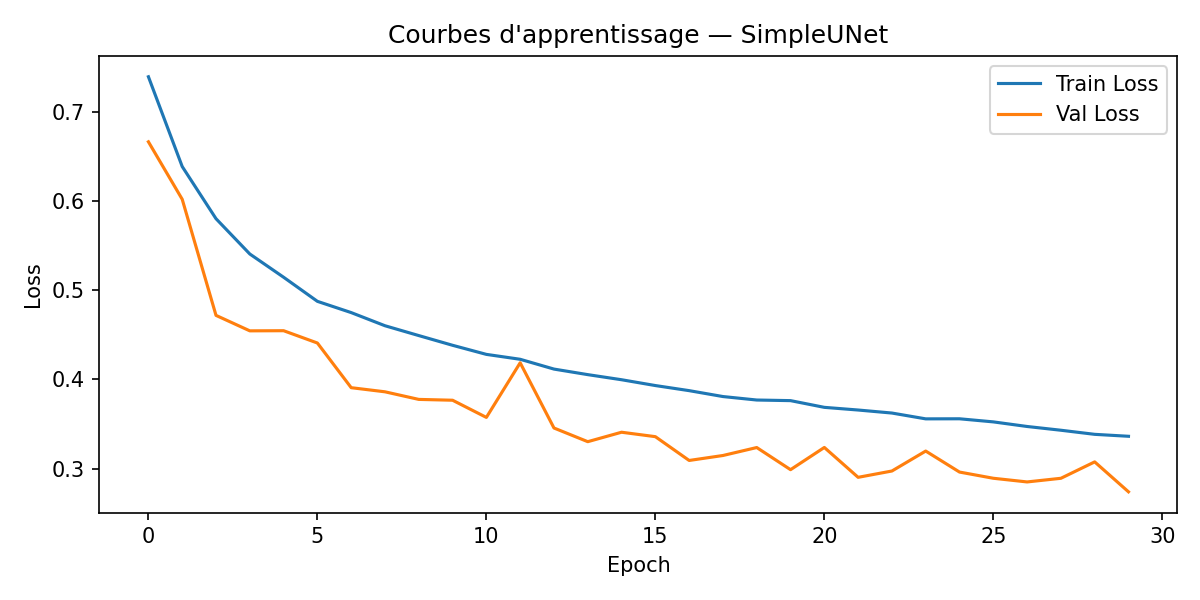
\includegraphics[width=0.8\textwidth]{learning_curves_SimpleUNet.png}
    \caption{Courbes d'apprentissage de la fonction de perte pour SimpleUNet.}
\end{figure}

\textbf{Analyse des courbes :} 
Les courbes montrent une diminution régulière et rapide de la perte d'entraînement. La perte de validation diminue parallèlement puis commence à osciller et stagner après une quinzaine d'epochs. Cela signale le début d'un sur-apprentissage (overfitting). L'Early Stopping permet d'interrompre l'entraînement avant que le modèle ne sur-apprenne excessivement sur le jeu de train et d'exporter les poids optimaux enregistrés au minimum de la loss de validation.

\subsubsection*{Évaluation et Matrice de Confusion}
Le modèle optimal évalué sur le jeu de test obtient un score de \textbf{mIoU = 0.7084} et un score de \textbf{mDice = 0.8164}.

\begin{figure}[H]
    \centering
    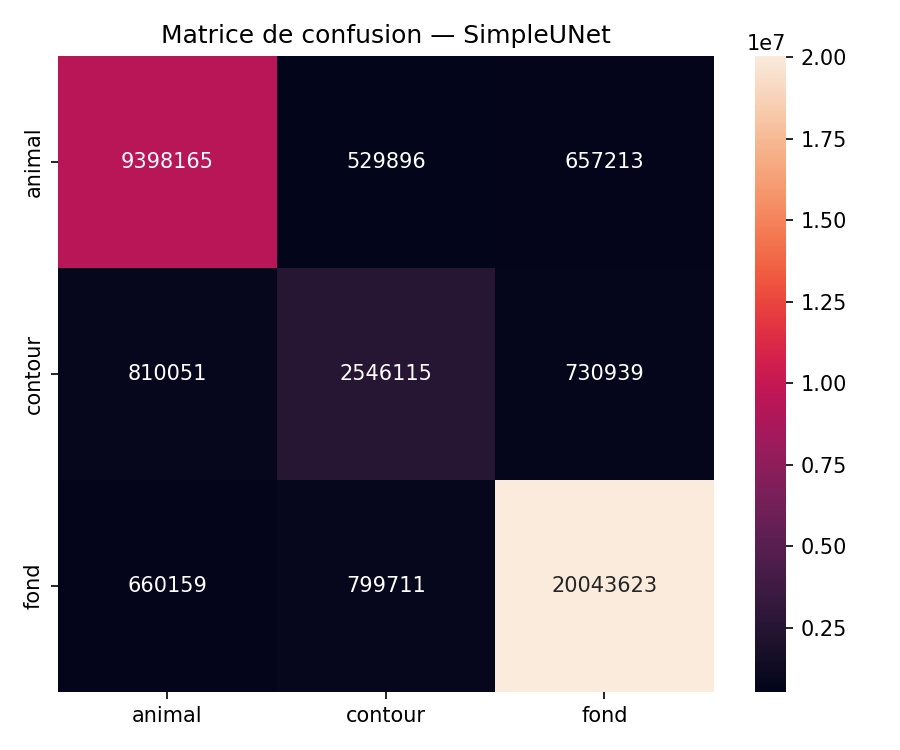
\includegraphics[width=0.65\textwidth]{confusion_matrix_SimpleUNet.png}
    \caption{Matrice de confusion normalisée des pixels pour le modèle SimpleUNet.}
\end{figure}

\textbf{Analyse des erreurs :} 
La matrice de confusion confirme que la classe des contours est la plus difficile à classifier (IoU individuelle de $0.470$, contre $0.780$ pour l'animal et $0.876$ pour le fond). On observe un chevauchement notable : une partie importante des pixels appartenant théoriquement au contour est prédite comme faisant partie de l'animal ou de l'arrière-plan. Les contours étant fins et minces, les réductions de résolution successives par Max Pooling altèrent l'information spatiale fine de ces limites, rendant la détection imprécise.

\newpage
\subsection{Partie 3 : Transfer Learning (TransferUNet)}
Pour pallier les limites du modèle de base, nous avons implémenté le modèle \texttt{TransferUNet}. Il utilise l'architecture pré-entraînée \textit{ResNet-34} (chargée avec les poids d'ImageNet) comme extracteur de caractéristiques (encodeur) et s'associe à un décodeur de segmentation avec Skip Connections. Nous étudions deux configurations distinctes :
\begin{enumerate}
    \item \textbf{TransferUNet (Frozen) :} L'encodeur ResNet-34 est gelé (\texttt{requires\_grad = False}). Seul le décodeur est entraîné.
    \item \textbf{TransferUNet (Fine-Tuned) :} L'ensemble du réseau est entraîné. Un taux d'apprentissage différentiel est utilisé : $10^{-4}$ pour l'encodeur ResNet-34 afin de préserver ses filtres généraux, et $10^{-3}$ pour le décodeur de segmentation.
\end{enumerate}

Le tableau suivant regroupe l'ensemble des résultats de synthèse mesurés sur notre environnement local (GPU NVIDIA avec accélération CUDA) :

\begin{table}[H]
\centering
\begin{tabular}{@{}lccccc@{}}
\toprule
\textbf{Modèle} & \textbf{mIoU} & \textbf{mDice} & \textbf{Nb Params} & \textbf{Temps/epoch} & \textbf{Inférence} \\ \midrule
SimpleUNet & 0.7084 & 0.8164 & 1,949,763 & $\sim$45s & 4.66 ms \\
TransferUNet (frozen) & 0.8008 & 0.8804 & 24,365,315 & $\sim$35s & 3.33 ms \\
TransferUNet (fine-tuned) & 0.8039 & 0.8825 & 24,365,315 & $\sim$80s & 3.18 ms \\ \bottomrule
\end{tabular}
\caption{Tableau comparatif des performances globales de segmentation sur le Test Set.}
\end{table}

Afin d'apporter une vision plus fine des performances pour chaque type de pixel, le tableau suivant détaille l'IoU et le coefficient de Dice classe par classe (Animal, Contour et Fond) pour l'ensemble des architectures testées :

\begin{table}[H]
\centering
\begin{tabular}{@{}lcccccc@{}}
\toprule
 & \multicolumn{2}{c}{\textbf{Animal}} & \multicolumn{2}{c}{\textbf{Contour}} & \multicolumn{2}{c}{\textbf{Fond}} \\ \cmidrule(lr){2-3} \cmidrule(lr){4-5} \cmidrule(lr){6-7}
\textbf{Modèle} & \textbf{IoU} & \textbf{Dice} & \textbf{IoU} & \textbf{Dice} & \textbf{IoU} & \textbf{Dice} \\ \midrule
SimpleUNet & 0.7796 & 0.8761 & 0.4700 & 0.6395 & 0.8756 & 0.9337 \\
TransferUNet (frozen) & 0.8818 & 0.9372 & 0.5818 & 0.7356 & 0.9388 & 0.9684 \\
TransferUNet (fine-tuned) & 0.8846 & 0.9388 & 0.5864 & 0.7393 & 0.9406 & 0.9694 \\ \bottomrule
\end{tabular}
\caption{Comparatif détaillé des performances par classe (IoU et Dice) sur le Test Set.}
\end{table}

De plus, nous présentons ci-dessous une comparaison visuelle qualitative sur six échantillons représentatifs du jeu de test. Cette visualisation permet de confronter directement les prédictions spatiales de chaque modèle avec les images originales et leurs masques cibles de vérité terrain (GT) :

\begin{figure}[H]
    \centering
    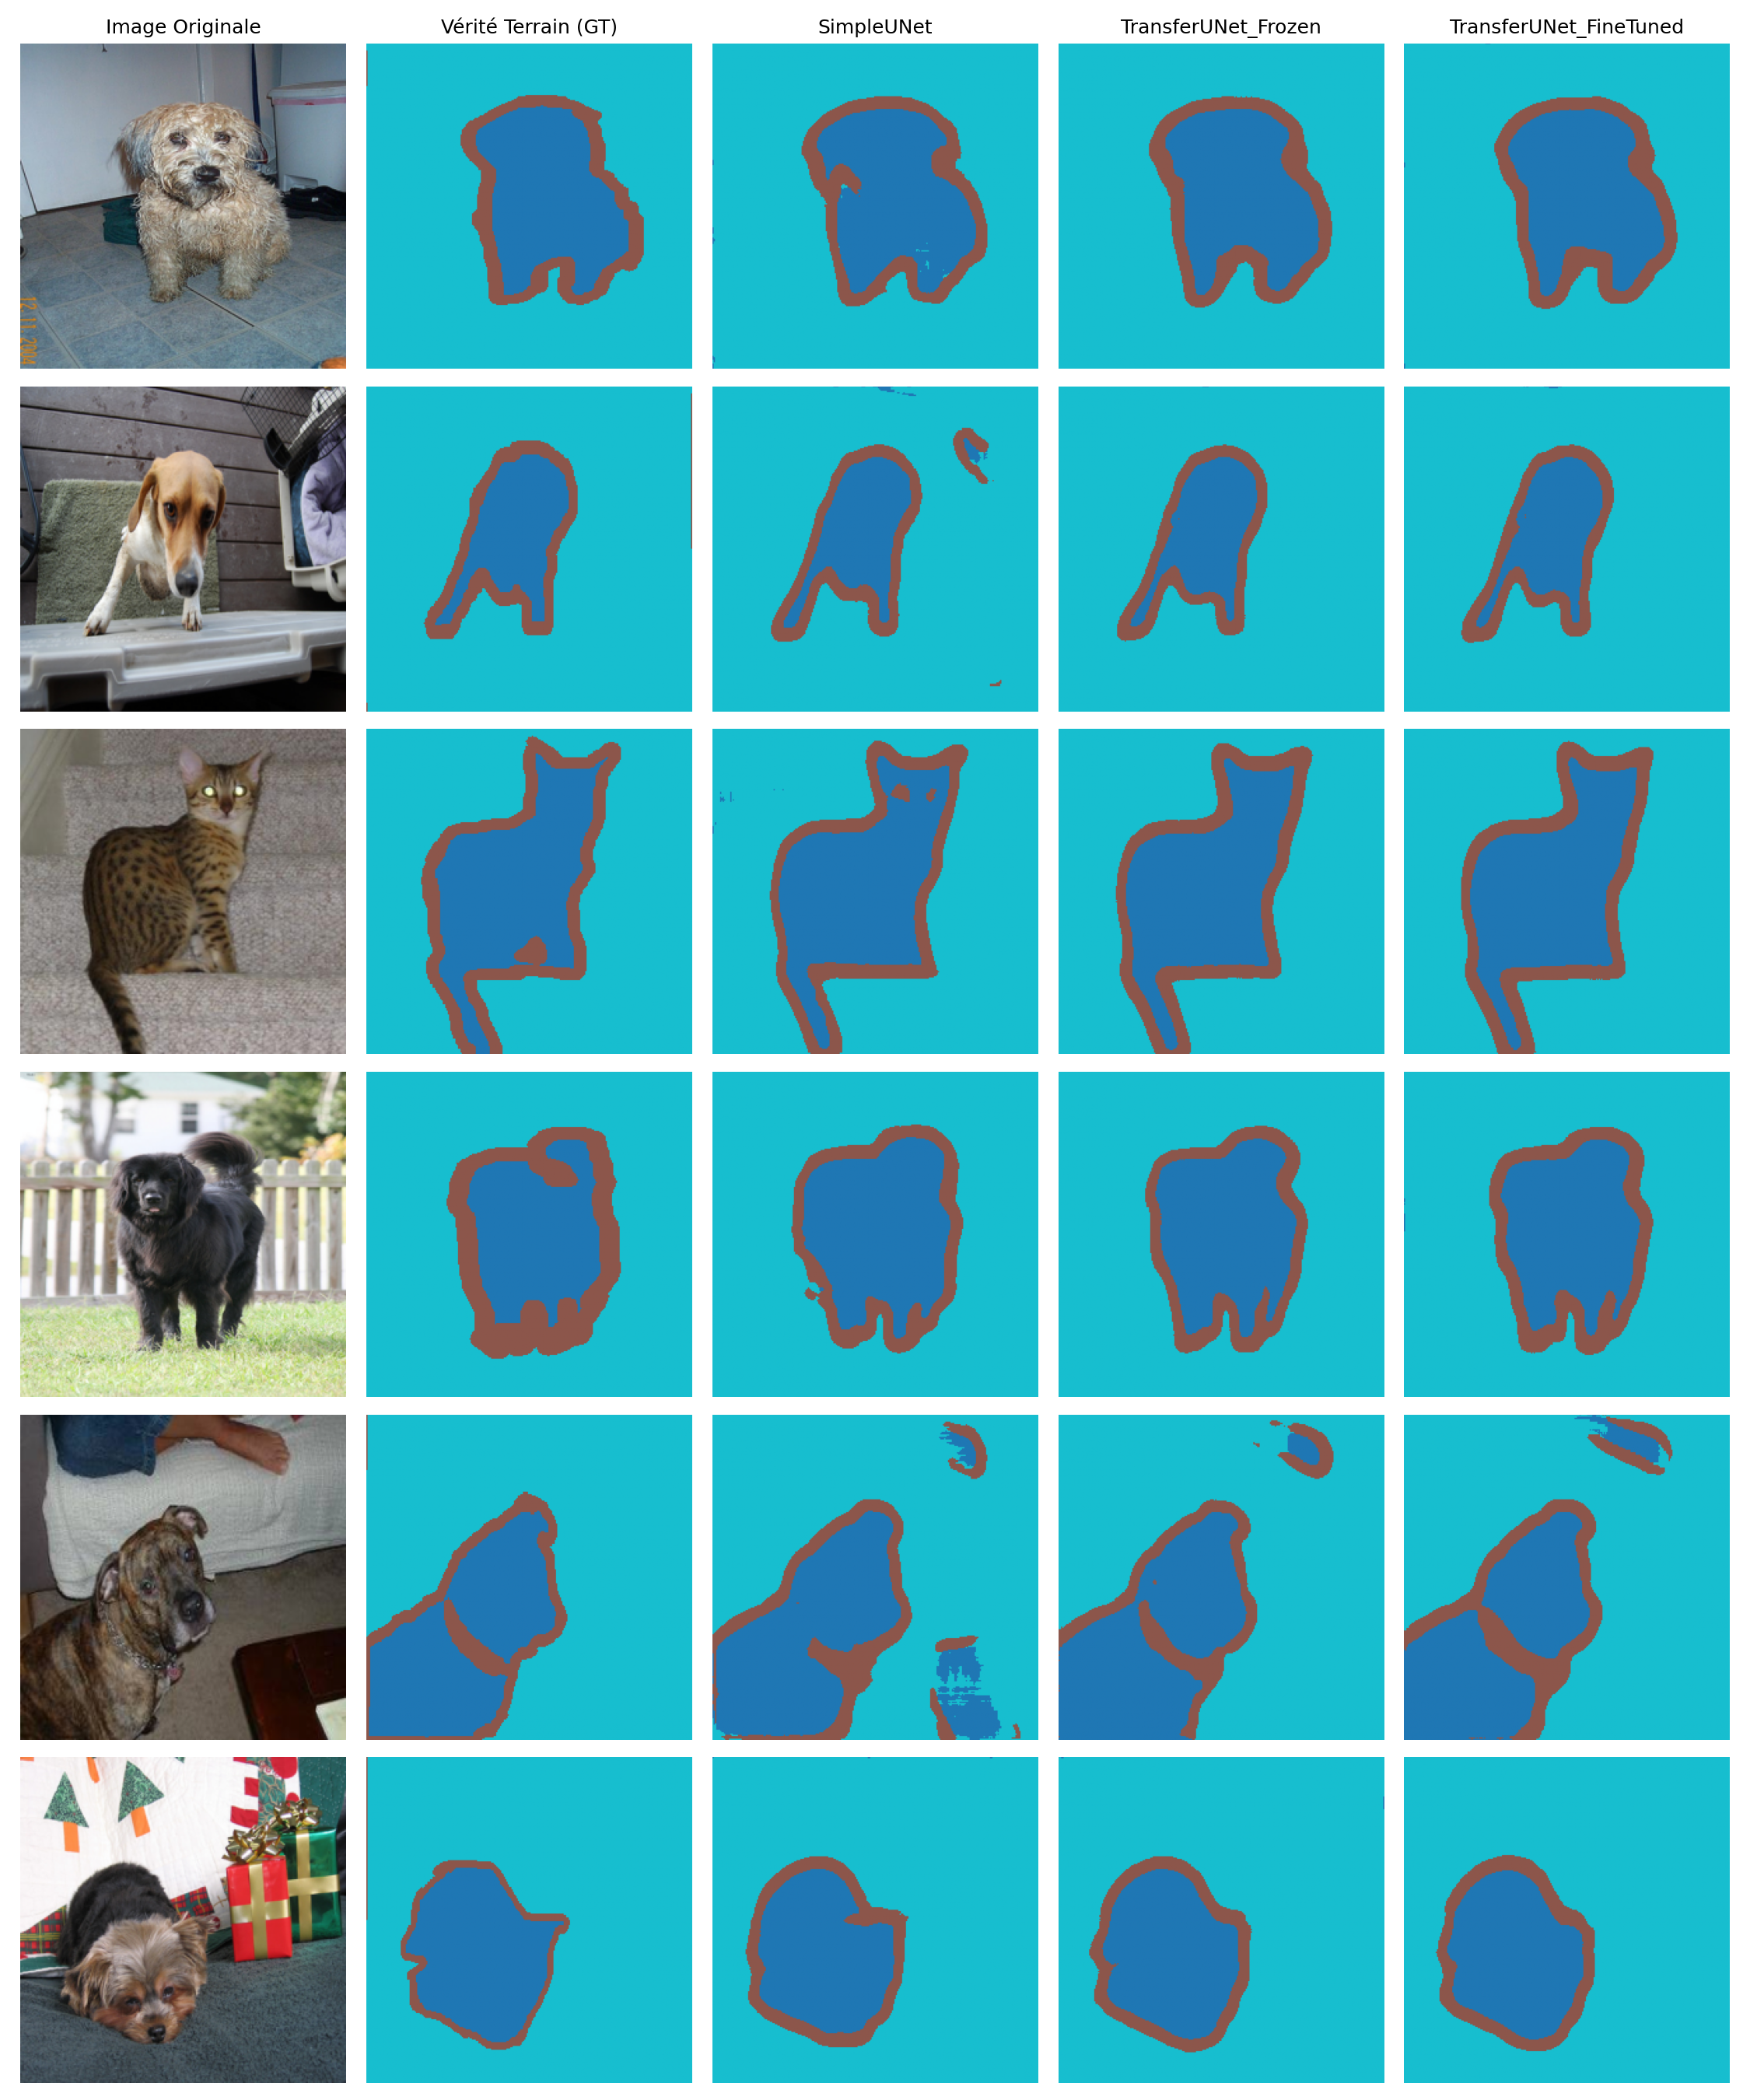
\includegraphics[width=1.0\textwidth]{predictions_comparison.png}
    \caption{Visualisation qualitative de 6 exemples d'évaluation sur le jeu de test. De gauche à droite : l'image originale, le masque de vérité terrain (GT), les prédictions du modèle SimpleUNet, du modèle TransferUNet (Frozen) et du modèle TransferUNet (Fine-Tuned).}
\end{figure}

\begin{figure}[H]
    \centering
    \begin{minipage}{0.48\textwidth}
        \centering
        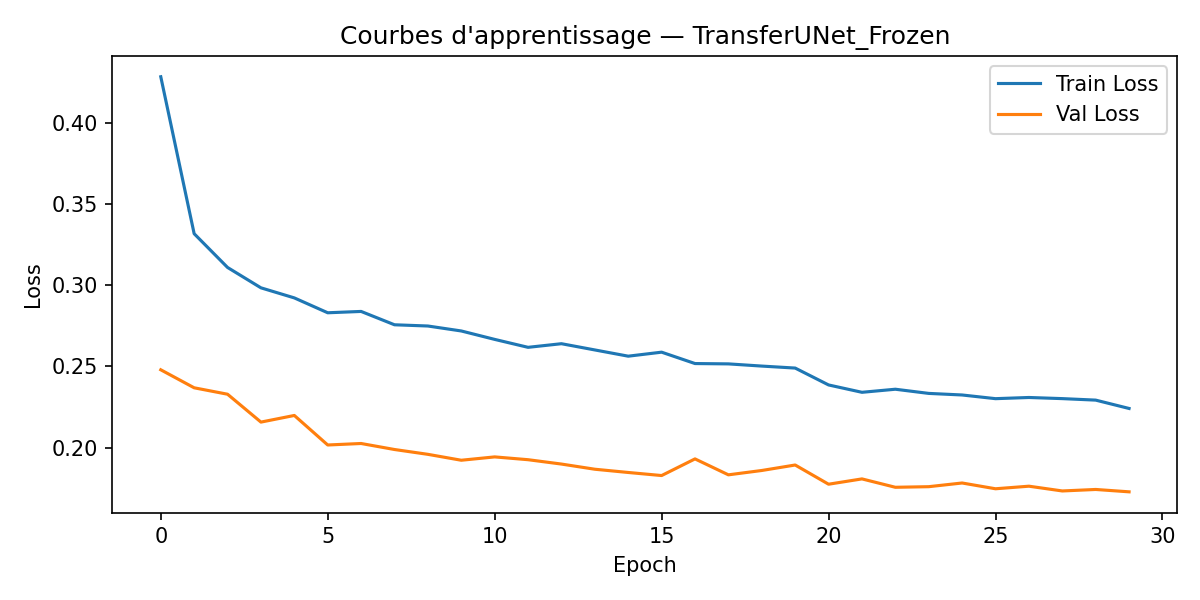
\includegraphics[width=\textwidth]{learning_curves_TransferUNet_Frozen.png}
        \caption{Courbes TransferUNet (Frozen)}
    \end{minipage}
    \hfill
    \begin{minipage}{0.48\textwidth}
        \centering
        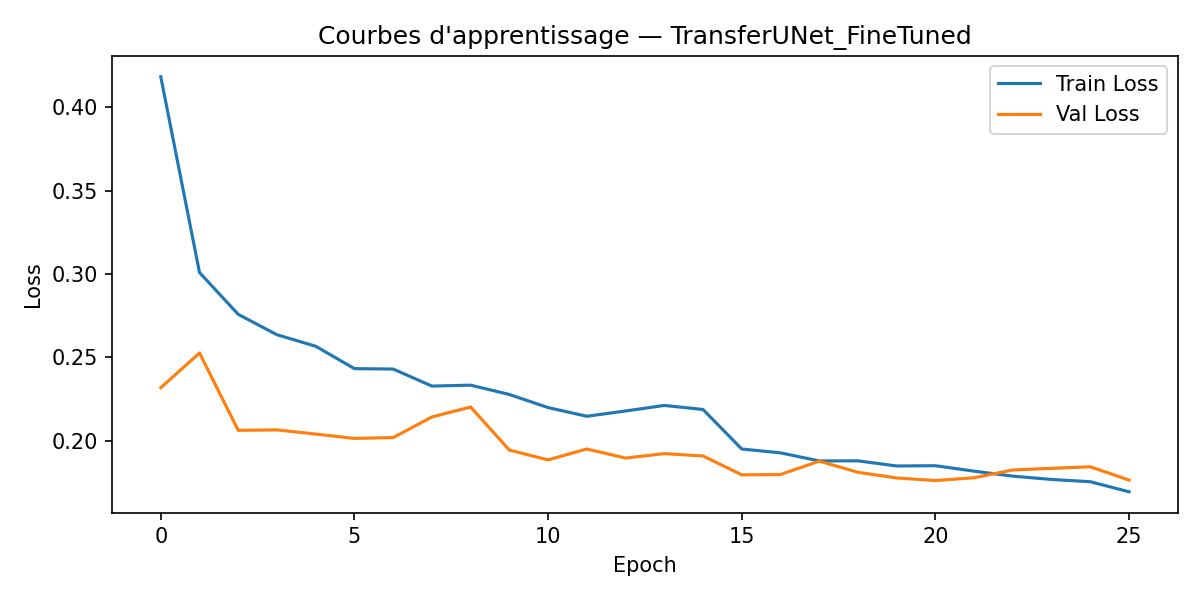
\includegraphics[width=\textwidth]{learning_curves_TransferUNet_FineTuned.png}
        \caption{Courbes TransferUNet (Fine-Tuned)}
    \end{minipage}
\end{figure}

\begin{figure}[H]
    \centering
    \begin{minipage}{0.48\textwidth}
        \centering
        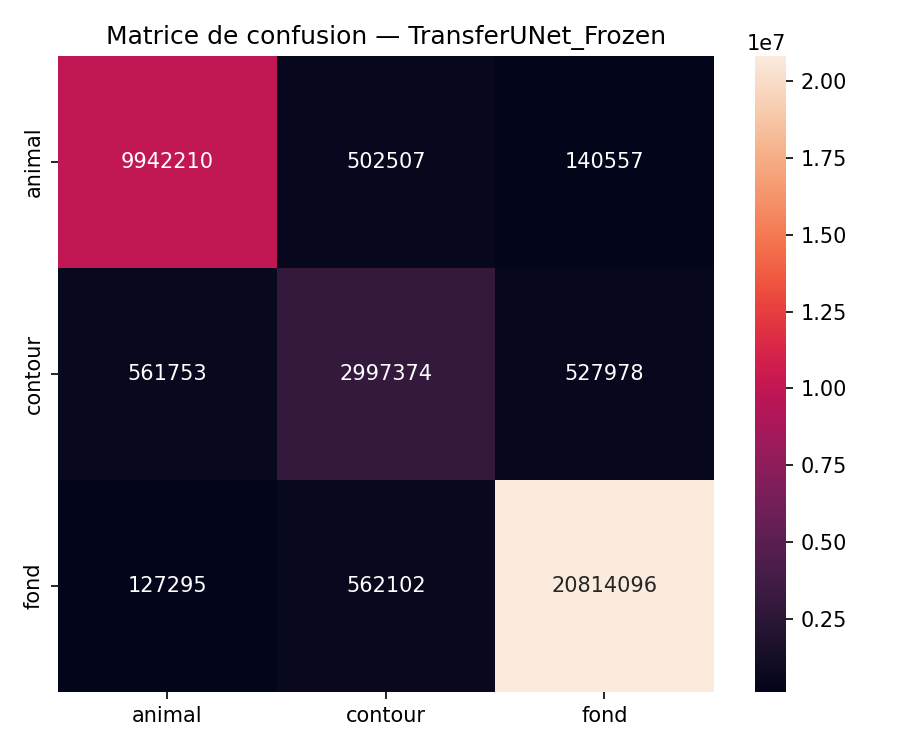
\includegraphics[width=0.9\textwidth]{confusion_matrix_TransferUNet_Frozen.png}
        \caption{Matrice TransferUNet (Frozen)}
    \end{minipage}
    \hfill
    \begin{minipage}{0.48\textwidth}
        \centering
        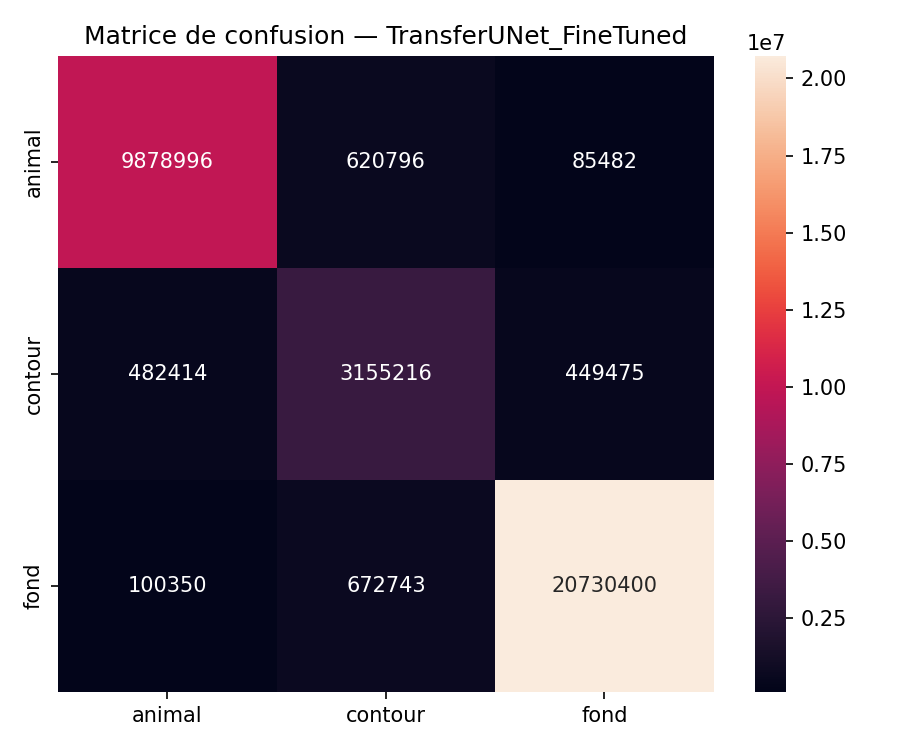
\includegraphics[width=0.9\textwidth]{confusion_matrix_TransferUNet_FineTuned.png}
        \caption{Matrice TransferUNet (Fine-Tuned)}
    \end{minipage}
\end{figure}

\textbf{Analyse comparative :}
\begin{itemize}
    \item \textbf{Performance métrique :} Le Transfer Learning apporte un gain de performance spectaculaire. Le mIoU passe d'environ $0.708$ (SimpleUNet) à plus de $0.800$. Cela s'explique par le fait que l'encodeur ResNet-34 a été pré-entraîné à extraire des primitives visuelles riches et robustes (bords, textures, contrastes) sur ImageNet, ce qui fournit des représentations de bien meilleure qualité au décodeur. Le fine-tuning complet (\texttt{Fine-Tuned}) améliore légèrement le mIoU ($0.8039$) par rapport à la version gelée ($0.8008$), mais au prix d'un coût de calcul nettement supérieur.
    \item \textbf{Vitesse d'entraînement :} Le modèle \texttt{TransferUNet (frozen)} est le plus rapide à entraîner ($\approx 35$ secondes par epoch). N'ayant pas à propager les gradients à travers les 21 millions de paramètres de l'encodeur, les calculs sont simplifiés et la convergence est plus rapide. Le \texttt{TransferUNet (fine-tuned)} est quant à lui le plus lent ($\approx 80$ secondes par epoch) car l'ensemble des 24 millions de paramètres nécessite un calcul de gradient à chaque itération.
    \item \textbf{Vitesse d'inférence :} De manière intéressante, les modèles basés sur ResNet-34 ont un temps d'inférence légèrement plus court ($\sim 3.0$ ms) que le \texttt{SimpleUNet} ($\sim 4.6$ ms). Bien que ResNet-34 compte dix fois plus de paramètres, ses couches convolutives et ses connexions résiduelles sont hautement optimisées au niveau matériel et par l'implémentation CUDA, ce qui accélère le flux d'inférence par rapport aux convolutions consécutives non résiduelles de notre SimpleUNet basique.
\end{itemize}

\newpage
% ==========================================
% CONCLUSION
% ==========================================
\section{Conclusion}
Ce travail pratique dédié à la segmentation sémantique d'images a mis en lumière des concepts clés en apprentissage profond appliqué à la vision par ordinateur. 

La conception d'un \texttt{SimpleUNet} à partir de zéro a permis de mettre en évidence la difficulté à traiter les classes géométriquement fines et minoritaires (comme les contours). Elle a également illustré le phénomène classique d'overfitting face à des architectures entraînées sur des volumes de données limités. 

L'introduction du \texttt{Transfer Learning} via un encodeur \texttt{ResNet-34} pré-entraîné a résolu ces limitations de manière flagrante, augmentant le mIoU de 10 points de pourcentage absolus. La comparaison a de plus mis en lumière un choix crucial lors de la mise en production de réseaux de neurones : la version "frozen" se révèle être le meilleur compromis, offrant des métriques quasi-optimales et un temps d'apprentissage réduit de moitié par rapport au fine-tuning complet.

\end{document}
